
%%%%%%%%%%%%%%%%%%%%%%%%%%%%%%%%%%%%%%%%%%%%%%%%%%%%%%%%%%%
\section{Object Manipulation With Hardware Robots}\label{sec:realExperiment}
%%%%%%%%%%%%%%%%%%%%%%%%%%%%%%%%%%%%%%%%%%%%%%%%%%%%%%%%%%%

  
\subsection{Environmental Setup}
Our experiments use centimeter-scale hardware systems called \emph{kilobots}.  While those are far larger than the micro scale devices we model, using kilobots allows us to emulate a variety of dynamics, while enabling a high degree of control over robot function, the environment, and data collection. The kilobot \cite{Rubenstein2012,rubenstein2014programmable} is a low-cost robot designed for testing collective algorithms with large numbers of robots. It is available commercially or as an open source platform~\cite{K-Team2015}.  Each robot is approximately 3 cm in diameter, 3 cm tall, and uses two vibration motors to move on a flat surface at speeds up to 1 cm/s.  Each robot has one ambient light sensor that is used to implement \emph{phototaxis},  moving towards a light source. 
In these experiments as shown in Fig.~\ref{fig:setup}, we used $n$=100 kilobots, a 1.5 m$\times$1.2 m whiteboard as the workspace, and eight 30W LED floodlights arranged 1.5 m above the plane of the table at the $\{N,NE,E,SE,S,SW,W,NW\}$ vertices of a 6 m square centered on the workspace. The lights were controlled using an Arduino Uno board connected to an 8 relay shield board.  Above the table, an overhead machine vision system tracks the position of the swarm. Laser-cut patterns for our neon green fiducial markers and our {\sc Matlab} tracking code are available at our github repository~\cite{Shahrokhi2015GitHubShapeControl}.
\begin{figure}
\begin{center}
	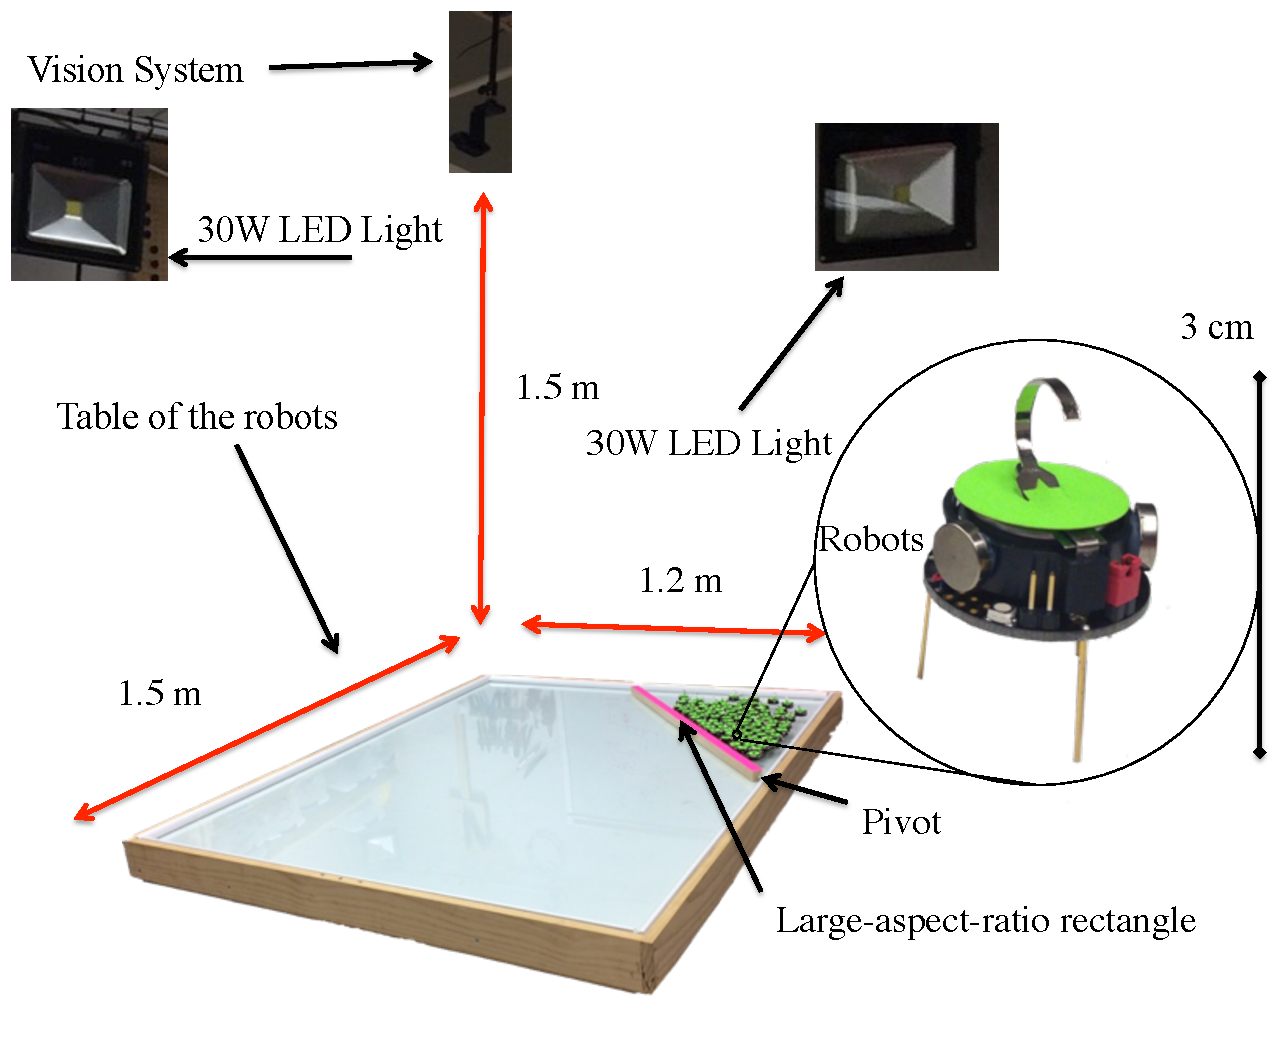
\includegraphics[width=\columnwidth]{SetUp.pdf}
\end{center}
\caption{\label{fig:setup}
Hardware platform:  table with 1.5$\times$1.2 m workspace, surrounded by eight remotely triggered 30W LED floodlights, with an overhead machine vision system.
}
\end{figure}
\subsection{Mean Control With Real Robots}

\begin{figure}
\begin{center}
	\includegraphics[width=\columnwidth]{Mean_Control_experiment.eps}
\end{center}
\caption{\label{fig:realMean}
Mean Control plot with kilobots.
}
\end{figure}

\begin{figure}
\begin{center}
	\includegraphics[width=\columnwidth]{XYMeanControl.eps}
\end{center}
\caption{\label{fig:meanRobotFig}
Mean Control experiment with kilobots.
}
\end{figure}

\subsection{Automated Object Manipulation}
\paragraph{Heuristics to Handle Outliers and Improve Performance}

The variance controller (eq XX) is a greedy algorithm that is susceptible to outliers. The controller in [x] failed in XX? trials, often because workspace obstacles made some robots unable to reach the object. The mean and covariance calculations (Eqs. Xx and XX) included all robots in the workspace. Robots that cannot reach the object due to obstacles skew these calculations. The state machine in Fig. 1 solves this problem by creating two states for the maze: either main or transfer. Each state has a set of regions representing a discretized visibility polygon. Whenever the object crosses a region boundary the state toggles. The main regions are generated by extending obstacles until they meet another obstacle. The transfer regions are perpendicular to obstacle boundaries, and act as a buffer between two main regions.
Figure 2 shows the regions for the main state. The object is in region 1. An indicator function is applied to Eqs. [equations for mean and variance] so only robots inside region 1 are counted.  This filtering increases experimental success because the mean calculation only includes nearby robots that can directly interact with the object. In the example, we want the robots to push the object to the right. Without filtering the robots, the orange star is the mean and the algorithm would instruct the robots to push the object southeast. The filtered mean is at the yellow star and the algorithm instructs the robots to push the object directly east. 
When the object leaves main region 1 the maze state switches to transfer. The transfer regions are shown in Fig. 3.  The object is in transfer region 0, so only robots in transfer region 0 are included in the mean and covariance calculations.  
This heuristic improves performance by XX.

\paragraph{Potential Fields for Swarm Management}

Unfortunately, when the swarm is in front of the object, control law XX pushes the object backwards.  To fix this, we implement a potential field approach [spong] that attracts the swarm to the intermediate goal, but repulses the swarm from in front of the object.
The repulsive potential field is centered at the object?s COM and is active for a radius ?0, but is implemented only when the swarm mean is within ? of the desired direction of motion (SYMBOL??)

PUT EQUATIONS HERE.

 In simulations, ? =  ?/2,  ?  = XX, ? = XX. Because the kilobot hardware experiments have a slower time constant, they use ? =  ?/2,  ?  = XX, ? = XX. 



\begin{figure}
\centering
\begin{overpic}[width=1\columnwidth]{experimentSnapShot.pdf}\end{overpic}
%\todo{I like the 'target' symbol, but it is not self-documenting.  We need a legend explaining the min and max variance ellipses, the goal region, the variance, the mean, the object COM, and the target mean position.  I think these are easiest to make in powerpoint.
%Please use the same color and line style for the variance min and max as you use in Figure 4.
%}
%{blockpushingImageWithMeanAndVarianceOverlay.png}
\caption{\label{fig:bigPictureMeanAndVarianceForSwarm} A swarm of robots, all controlled by a uniform force field, can be effectively controlled by a hybrid controller that knows only the first and second moments of the robot distribution.  Here is a swarm of hardware robots(kilobots) that pushes a green block toward the goal. See video attachment~\cite{ShivaVideo2015}.}
\end{figure}